%
% Modelo de Dados
%
\section{Modelo de Dados}\label{sec31}



% Modelo EA
\subsection{Modelo Entidade-Associação}\label{subsec311}

\begin{figure}[H]
	\hspace*{-2,5cm}
	\centering
	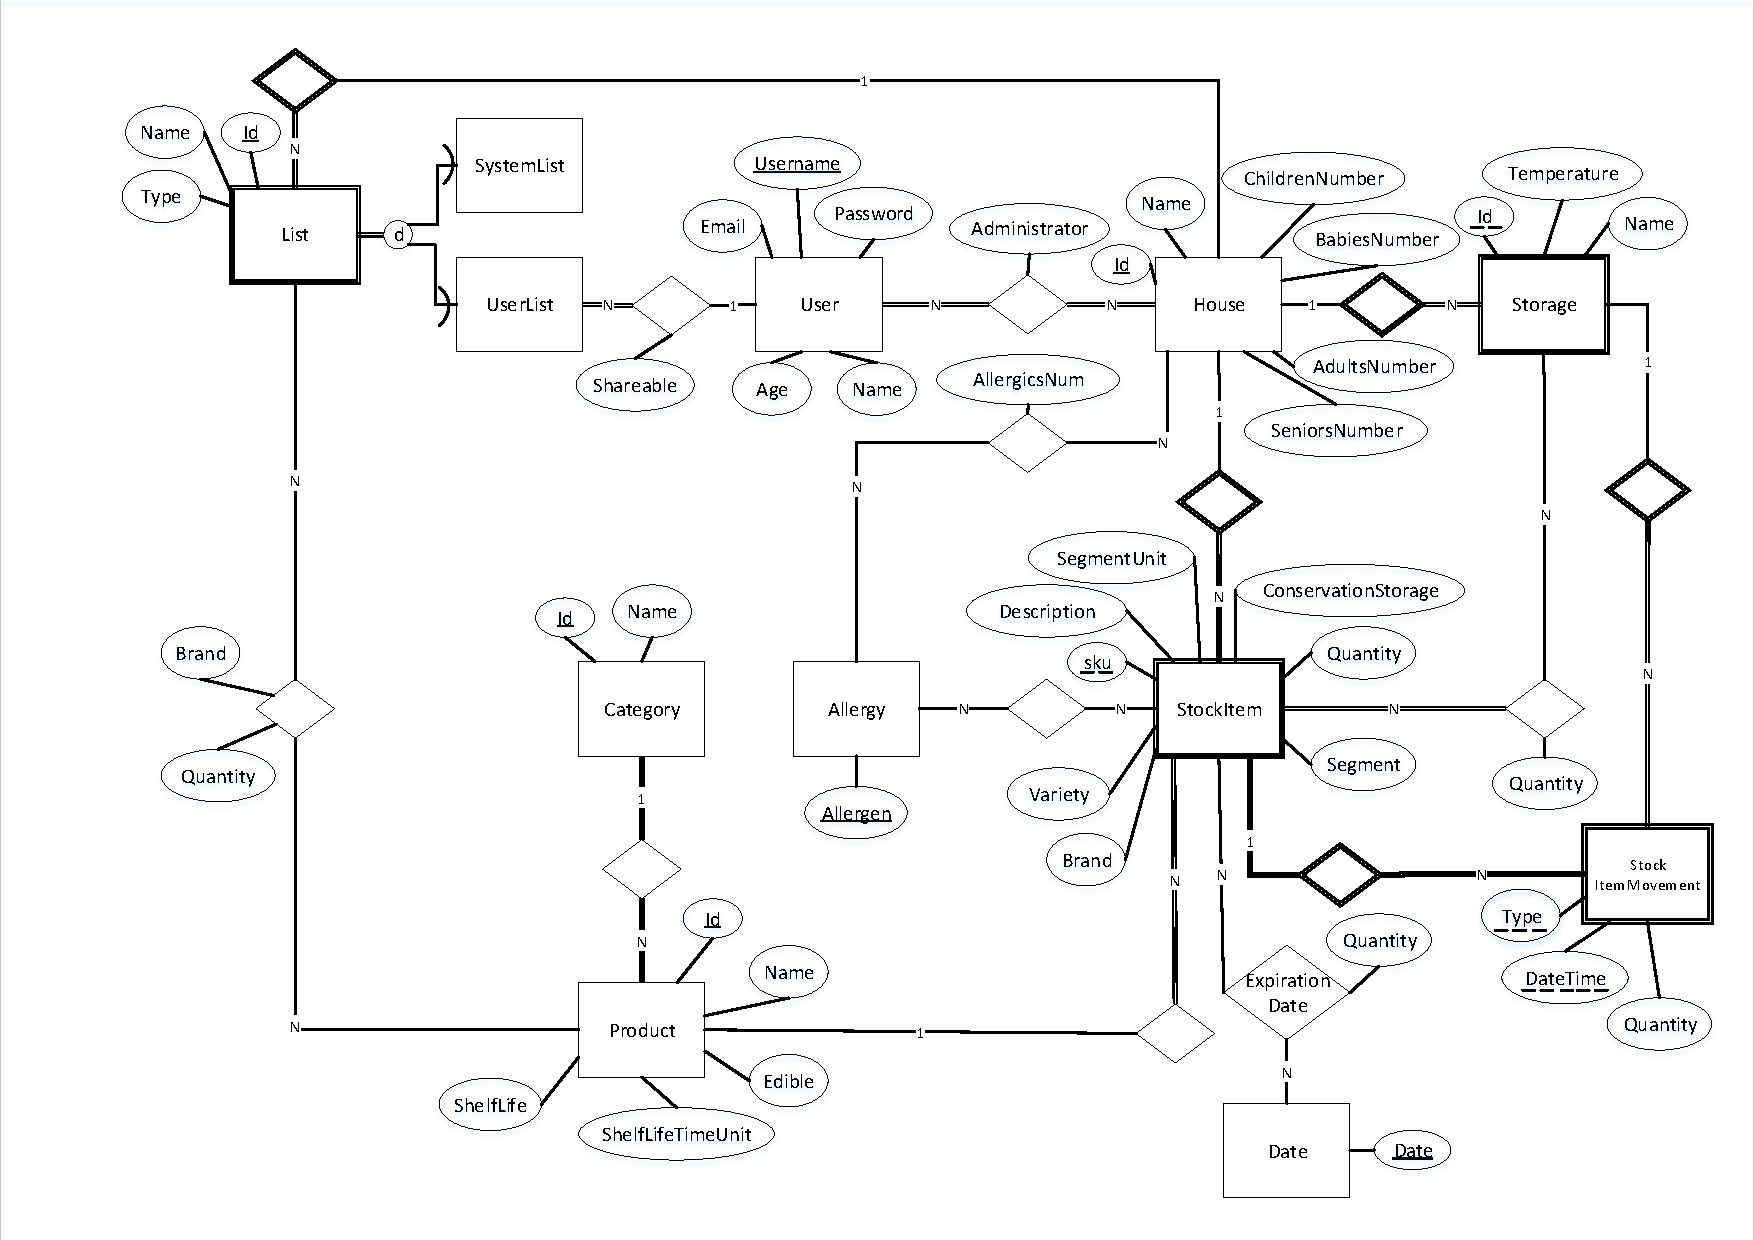
\includegraphics[width=20cm,height=15cm,scale=1]{./files/EA.pdf}
	\caption{Modelo Entidade-Associação}
	\label{modelo-ea}
\end{figure}

% Domínio dos Atributos
\subsection{Domínio dos Atributos}\label{subsec313}
\raggedbottom
% House
\begin{table} [H]
	\centering
	\caption{Domínio dos Atributos da Entidade House.} \vspace{2mm}
	\label{tab-dominio-atributos-house}
	\resizebox{\textwidth}{!}{%
		\begin{tabular}{|c|c|C{2.5cm}|C{2.7cm}|C{3.6cm}|C{2.3cm}|}
			\hline
			\textbf{Entidade} & \textbf{Atributo} & \textbf{Domínio} & \textbf{Tipo Variável (PostgreSQL)} & \textbf{Restrições} & \textbf{Nullable}\\ \hline
			\multirow{6}{*}{House} & house\_id & Número inteiro auto-incrementado & bigserial & - & não\\ \cline{2-6}
			& house\_name & Cadeia de caracteres de comprimento variável & character varying(35) & até 35 caracteres & não\\ \cline{2-6}
			& house\_characteristics & Objeto \acrshort{json} & json & - & não\\ \hline
		\end{tabular}
	}
\end{table}

% User
\begin{table} [H]
	\centering
	\caption{Domínio dos Atributos da Entidade User.} \vspace{2mm}
	\label{tab-dominio-atributos-user}
	\resizebox{\textwidth}{!}{%
		\begin{tabular}{|c|c|C{2.5cm}|C{2.7cm}|C{3.6cm}|C{2.3cm}|}
			\hline
			\textbf{Entidade} & \textbf{Atributo} & \textbf{Domínio} & \textbf{Tipo Variável (PostgreSQL)} & \textbf{Restrições} & \textbf{Nullable}\\ \hline
			\multirow{5}{*}{User} & user\_username & Cadeia de caracteres de comprimento variável & character varying(30) & até 30 caracteres & não\\ \cline{2-6}
			& user\_email & Cadeia de caracteres de comprimento variável & character varying(254) & até 254 caracteres & não\\ \cline{2-6}
			& user\_age & Número inteiro & smallint & user\_age in [0, 150] & não\\ \cline{2-6}
			& user\_name & Cadeia de caracteres de comprimento variável & character varying(70) & até 70 caracteres & não\\ \cline{2-6}
			& user\_password & Cadeia de caracteres de comprimento variável & character varying(50) & até 50 caracteres & não\\ \hline
		\end{tabular}
	}
\end{table}

% Allergy
\begin{table} [H]
	\centering
	\caption{Domínio dos Atributos da Entidade Allergy.} \vspace{2mm}
	\label{tab-dominio-atributos-allergy}
	\resizebox{\textwidth}{!}{%
		\begin{tabular}{|c|c|C{2.5cm}|C{2.7cm}|C{3.6cm}|C{2.3cm}|}
			\hline
			\textbf{Entidade} & \textbf{Atributo} & \textbf{Domínio} & \textbf{Tipo Variável (PostgreSQL)} & \textbf{Restrições} & \textbf{Nullable}\\ \hline
			{Allergy} & allergy\_allergen & Cadeia de caracteres de comprimento variável & character varying(75) & até 75 caracteres & não\\ \hline
		\end{tabular}
	}
\end{table}


% Recipe
\begin{table} [H]
	\centering
	\caption{Domínio dos Atributos da Entidade Recipe.} \vspace{2mm}
	\label{tab-dominio-atributos-recipe}
	\resizebox{\textwidth}{!}{%
		\begin{tabular}{|c|c|C{2.5cm}|C{2.7cm}|C{3.6cm}|C{2.3cm}|}
			\hline
			\textbf{Entidade} & \textbf{Atributo} & \textbf{Domínio} & \textbf{Tipo Variável (PostgreSQL)} & \textbf{Restrições} & \textbf{Nullable}\\ \hline
			\multirow{9}{*}{Recipe} & recipe\_id & Número inteiro auto-incrementado & bigserial & - & não\\ \cline{2-6}
			& recipe\_name & Cadeia de caracteres de comprimento variável & character varying(35) & até 35 caracteres & não\\ \cline{2-6}
			& recipe\_instructions & Cadeia de caracteres de comprimento variável & text & - & não\\ \cline{2-6}
			& recipe\_difficulty & Cadeia de caracteres de comprimento variável & character varying(9) & recipe\_difficulty in ['easy', 'average', 'difficult'] & sim\\ \cline{2-6}
			& recipe\_time & Número inteiro & smallint & recipe\_time \textgreater{} 0 & sim\\ \cline{2-6}
			& recipe\_servings & Número inteiro & smallint & recipe\_servings \textgreater{} 0 & sim\\ \cline{2-6}
			& recipe\_cuisine & Cadeia de caracteres de comprimento variável & character varying(35) & até 35 caracteres & sim\\ \cline{2-6}
			& recipe\_dishType & Cadeia de caracteres de comprimento variável & character varying(35) & até 35 caracteres & sim\\ \cline{2-6}
			& recipe\_type & Cadeia de caracteres de comprimento variável & character varying(7) & recipe\_type  in ['system', 'user'] & não\\ \hline
		\end{tabular}
	}
\end{table}

% System Recipe
\begin{table} [H]
	\centering
	\caption{Domínio dos Atributos da Entidade SystemRecipe.} \vspace{2mm}
	\label{tab-dominio-atributos-systemRecipe}
	\resizebox{\textwidth}{!}{%
		\begin{tabular}{|c|c|C{2.5cm}|C{2.7cm}|C{3.6cm}|C{2.3cm}|}
			\hline
			\textbf{Entidade} & \textbf{Atributo} & \textbf{Domínio} & \textbf{Tipo Variável (PostgreSQL)} & \textbf{Restrições} & \textbf{Nullable}\\ \hline
			{System Recipe} & recipe\_id & Número inteiro & bigint & recipe\_id \textgreater{} 0 & não\\ \hline
		\end{tabular}
	}
\end{table}

% User Recipe
\begin{table} [H]
	\centering
	\caption{Domínio dos Atributos da Entidade UserRecipe.} \vspace{2mm}
	\label{tab-dominio-atributos-userRecipe}
	\resizebox{\textwidth}{!}{%
		\begin{tabular}{|c|c|C{2.5cm}|C{2.7cm}|C{3.6cm}|C{2.3cm}|}
			\hline
			\textbf{Entidade} & \textbf{Atributo} & \textbf{Domínio} & \textbf{Tipo Variável (PostgreSQL)} & \textbf{Restrições} & \textbf{Nullable}\\ \hline
			\multirow{2}{*}{User Recipe} & recipe\_id & Número inteiro & bigint & recipe\_id \textgreater{} 0 & não\\ \cline{2-6}
			& user\_username & Cadeia de caracteres de comprimento variável & character varying(30) & até 30 caracteres & não\\ \hline
		\end{tabular}
	}
\end{table}

% Shared Recipe
\begin{table} [H]
	\centering
	\caption{Domínio dos Atributos da Entidade SharedRecipe.} \vspace{2mm}
	\label{tab-dominio-atributos-sharedRecipe}
	\resizebox{\textwidth}{!}{%
		\begin{tabular}{|c|c|C{2.5cm}|C{2.7cm}|C{3.6cm}|C{2.3cm}|}
			\hline
			\textbf{Entidade} & \textbf{Atributo} & \textbf{Domínio} & \textbf{Tipo Variável (PostgreSQL)} & \textbf{Restrições} & \textbf{Nullable}\\ \hline
			\multirow{2}{*}{Shared Recipe} & recipe\_id & Número inteiro & bigint & recipe\_id \textgreater{} 0 & não\\ \cline{2-6}
			& user\_username & Cadeia de caracteres de comprimento variável & character varying(30) & até 30 caracteres & não\\ \hline
		\end{tabular}
	}
\end{table}

% List
\begin{table} [H]
	\centering
	\caption{Domínio dos Atributos da Entidade List.} \vspace{2mm}
	\label{tab-dominio-atributos-list}
	\resizebox{\textwidth}{!}{%
		\begin{tabular}{|c|c|C{2.5cm}|C{2.7cm}|C{3.6cm}|C{2.3cm}|}
			\hline
			\textbf{Entidade} & \textbf{Atributo} & \textbf{Domínio} & \textbf{Tipo Variável (PostgreSQL)} & \textbf{Restrições} & \textbf{Nullable}\\ \hline
			\multirow{4}{*}{List} & house\_id & Número inteiro & bigint & house\_id \textgreater{} 0 & não\\ \cline{2-6}
			& list\_id & Número inteiro auto-incrementado & smallint & - & não\\ \cline{2-6}
			& list\_name & Cadeia de caracteres de comprimento variável & character varying(35) & até 35 caracteres & não\\ \cline{2-6}
			& list\_type & Cadeia de caracteres de comprimento variável & character varying(7) & list\_type  in ['system', 'user'] & não\\ \hline
		\end{tabular}
	}
\end{table}

% System List
\begin{table} [H]
	\centering
	\caption{Domínio dos Atributos da Entidade SystemList.} \vspace{2mm}
	\label{tab-dominio-atributos-systemList}
	\resizebox{\textwidth}{!}{%
		\begin{tabular}{|c|c|C{2.5cm}|C{2.7cm}|C{3.6cm}|C{2.3cm}|}
			\hline
			\textbf{Entidade} & \textbf{Atributo} & \textbf{Domínio} & \textbf{Tipo Variável (PostgreSQL)} & \textbf{Restrições} & \textbf{Nullable}\\ \hline
			\multirow{2}{*}{System List} & house\_id & Número inteiro & bigint & house\_id \textgreater{} 0 & não\\ \cline{2-6}
			& list\_id & Número inteiro & smallint & list\_id \textgreater{} 0 & não\\ \hline
		\end{tabular}
	}
\end{table}

% User List
\begin{table} [H]
	\centering
	\caption{Domínio dos Atributos da Entidade UserList.} \vspace{2mm}
	\label{tab-dominio-atributos-userList}
	\resizebox{\textwidth}{!}{%
		\begin{tabular}{|c|c|C{2.5cm}|C{2.7cm}|C{3.6cm}|C{2.3cm}|}
			\hline
			\textbf{Entidade} & \textbf{Atributo} & \textbf{Domínio} & \textbf{Tipo Variável (PostgreSQL)} & \textbf{Restrições} & \textbf{Nullable}\\ \hline
			\multirow{4}{*}{User List} & house\_id & Número inteiro & bigint & house\_id \textgreater{} 0 & não\\ \cline{2-6}
			& list\_id & Número inteiro & smallint & list\_id \textgreater{} 0 & não\\ \cline{2-6}
			& user\_username & Cadeia de caracteres de comprimento variável & character varying(30) & até 30 caracteres & não\\ \cline{2-6}
			& list\_shareable & Booleano & boolean & - & sim\\ \hline
		\end{tabular}
	}
\end{table}

% Category
\begin{table} [H]
	\centering
	\caption{Domínio dos Atributos da Entidade Category.} \vspace{2mm}
	\label{tab-dominio-atributos-category}
	\resizebox{\textwidth}{!}{%
		\begin{tabular}{|c|c|C{2.5cm}|C{2.7cm}|C{3.6cm}|C{2.3cm}|}
			\hline
			\textbf{Entidade} & \textbf{Atributo} & \textbf{Domínio} & \textbf{Tipo Variável (PostgreSQL)} & \textbf{Restrições} & \textbf{Nullable}\\ \hline
			\multirow{2}{*}{Category} & category\_id & Número inteiro auto-incrementado & serial & - & não\\ \cline{2-6}
			& category\_name & Cadeia de caracteres de comprimento variável & character varying(35) & até 35 caracteres & não\\ \hline
		\end{tabular}
	}
\end{table}

% Product
\begin{table} [H]
	\centering
	\caption{Domínio dos Atributos da Entidade Product.} \vspace{2mm}
	\label{tab-dominio-atributos-product}
	\resizebox{\textwidth}{!}{%
		\begin{tabular}{|c|c|C{2.5cm}|C{2.7cm}|C{3.8cm}|C{2cm}|}
			\hline
			\textbf{Entidade} & \textbf{Atributo} & \textbf{Domínio} & \textbf{Tipo Variável (PostgreSQL)} & \textbf{Restrições} & \textbf{Nullable}\\ \hline
			\multirow{6}{*}{Product} & category\_id & Número inteiro & integer & category\_id \textgreater{} 0 & não\\ \cline{2-6}
			& product\_id & Número inteiro auto-incrementado & integer & - & não\\ \cline{2-6}
			& product\_name & Cadeia de caracteres de comprimento variável & character varying(35) & até 35 caracteres & não\\ \cline{2-6}
			& product\_edible & Booleano & boolean & - & não\\ \cline{2-6}
			& product\_shelfLife & Número inteiro & smallint & product\_shelfLife \textgreater{} 0 & não\\ \cline{2-6}
			& product\_shelfLifeTimeUnit & Cadeia de caracteres de comprimento variável & character varying(5) & product\_shelfLifeTimeUnit in ['day', 'week', 'month', 'year'] & não\\ \hline
		\end{tabular}
	}
\end{table}

% StockItem
\begin{table} [H]
	\centering
	\caption{Domínio dos Atributos da Entidade StockItem.} \vspace{2mm}
	\label{tab-dominio-atributos-stockItem}
	\resizebox{\textwidth}{!}{%
		\begin{tabular}{|c|c|C{2.5cm}|C{2.7cm}|C{3.6cm}|C{2cm}|}
			\hline
			\textbf{Entidade} & \textbf{Atributo} & \textbf{Domínio} & \textbf{Tipo Variável (PostgreSQL)} & \textbf{Restrições} & \textbf{Nullable}\\ \hline
			\multirow{11}{*}{StockItem} & house\_id & Número inteiro & bigint & house\_id \textgreater{} 0 & não\\ \cline{2-6}
			& stockItem\_sku & Cadeia de caracteres de comprimento variável & character varying(128) & até 128 caracteres & não\\ \cline{2-6}
			& category\_id & Número inteiro & integer & category\_id \textgreater{} 0 & não\\ \cline{2-6}
			& product\_id & Número inteiro & integer & product\_id \textgreater{} 0 & não\\ \cline{2-6}
			& stockItem\_brand & Cadeia de caracteres de comprimento variável & character varying(35) & até 35 caracteres & não\\ \cline{2-6}
			& stockItem\_segment & Número décimal & real & stockItem\_segment \textgreater{} 0 & não\\ \cline{2-6}
			& stockItem\_variety & Cadeia de caracteres de comprimento variável & character varying(35) & até 35 caracteres & não\\ \cline{2-6}
			& stockItem\_quantity & Número inteiro & smallint & stockItem\_quantity \textgreater{} 0 & não\\ \cline{2-6}
			& stockItem\_segmentUnit & Cadeia de caracteres de comprimento variável & character varying(5) & stockItem\_segmentUnit in ['kg', 'dag', 'hg', 'g', 'dg', 'cg', 'mg', 'kl', 'hl', 'dal', 'l', 'dl', 'cl', 'ml', 'oz', 'lb', 'pt', 'fl oz', 'units'] & não\\ \cline{2-6}
			& stockItem\_description & Cadeia de caracteres de comprimento variável & text & - & sim\\ \cline{2-6}
			& stockItem\_conservationStorage & Cadeia de caracteres de comprimento variável & character varying(128) & até 128 caracteres & não\\ \hline
		\end{tabular}
	}
\end{table}
	
% Ingredient
\begin{table} [H]
	\centering
	\caption{Domínio dos Atributos da Entidade Ingredient.} \vspace{2mm}
	\label{tab-dominio-atributos-ingredient}
	\resizebox{\textwidth}{!}{%
		\begin{tabular}{|c|c|C{2.5cm}|C{2.7cm}|C{3.6cm}|C{2.3cm}|}
			\hline
			\textbf{Entidade} & \textbf{Atributo} & \textbf{Domínio} & \textbf{Tipo Variável (PostgreSQL)} & \textbf{Restrições} & \textbf{Nullable}\\ \hline
			\multirow{5}{*}{Ingredient} & recipe\_id & Número inteiro & integer & recipe\_id \textgreater{} 0 & não\\ \cline{2-6}
			& category\_id & Número inteiro & integer & category\_id \textgreater{} 0 & não\\ \cline{2-6}
			& product\_id & Número inteiro & integer & product\_id \textgreater{} 0 & não\\ \cline{2-6}
			& ingredient\_quantity & Número inteiro & integer & ingredient\_quantity \textgreater{} 0 & não\\ \cline{2-6}
			& ingredient\_quantityUnit & Cadeia de caracteres de comprimento variável & character varying(5) & ingredient\_quantityUnit in ['kg', 'dag', 'hg', 'g', 'dg', 'cg', 'mg', 'kl', 'hl', 'dal', 'l', 'dl', 'cl', 'ml', 'oz', 'lb', 'pt', 'fl oz', 'units'] & não\\ \hline
		\end{tabular}
	}
\end{table}

% Storage
\begin{table} [H]
	\centering
	\caption{Domínio dos Atributos da Entidade Storage.} \vspace{2mm}
	\label{tab-dominio-atributos-storage}
	\resizebox{\textwidth}{!}{%
		\begin{tabular}{|c|c|C{2.5cm}|C{2.7cm}|C{3.6cm}|C{2.3cm}|}
			\hline
			\textbf{Entidade} & \textbf{Atributo} & \textbf{Domínio} & \textbf{Tipo Variável (PostgreSQL)} & \textbf{Restrições} & \textbf{Nullable}\\ \hline
			\multirow{4}{*}{Storage} & house\_id & Número inteiro & bigint & house\_id \textgreater{} 0 & não\\ \cline{2-6}
			& storage\_id & Número inteiro auto-incrementado & smallint & - & não\\ \cline{2-6}
			& storage\_name & Cadeia de caracteres de comprimento variável & character varying(35) & até 35 caracteres & não\\ \cline{2-6}
			& storage\_temperature & Intervalo de números decimais & numrange & - & não\\ \hline
		\end{tabular}
	}
\end{table}

% User House
\begin{table} [H]
	\centering
	\caption{Domínio dos Atributos da Entidade UserHouse.} \vspace{2mm}
	\label{tab-dominio-atributos-userHouse}
	\resizebox{\textwidth}{!}{%
		\begin{tabular}{|c|c|C{2.5cm}|C{2.7cm}|C{3.6cm}|C{2.3cm}|}
			\hline
			\textbf{Entidade} & \textbf{Atributo} & \textbf{Domínio} & \textbf{Tipo Variável (PostgreSQL)} & \textbf{Restrições} & \textbf{Nullable}\\ \hline
			\multirow{3}{*}{UserHouse} & house\_id & Número inteiro & bigint & house\_id \textgreater{} 0 & não\\ \cline{2-6}
			& user\_username & Cadeia de caracteres de comprimento variável & character varying(30) & até 30 caracteres & não\\ \cline{2-6}
			& userHouse\_administrator & Booleano & boolean & - & sim\\ \hline
		\end{tabular}
	}
\end{table}

% StockItem Storage
\begin{table} [H]
	\centering
	\caption{Domínio dos Atributos da Entidade StockItemStorage.} \vspace{2mm}
	\label{tab-dominio-atributos-stockItemStorage}
	\resizebox{\textwidth}{!}{%
		\begin{tabular}{|c|c|C{2.3cm}|C{2.7cm}|C{3.6cm}|C{2cm}|}
			\hline
			\textbf{Entidade} & \textbf{Atributo} & \textbf{Domínio} & \textbf{Tipo Variável (PostgreSQL)} & \textbf{Restrições} & \textbf{Nullable}\\ \hline
			\multirow{4}{*}{StockItemStorage} & house\_id & Número inteiro & bigint & house\_id \textgreater{} 0 & não\\ \cline{2-6}
			& stockItem\_sku & Cadeia de caracteres de comprimento variável & character varying(128) & até 128 caracteres & não\\ \cline{2-6}
			& storage\_id & Número inteiro & smallint & storage\_id \textgreater{} 0 & não\\ \cline{2-6}
			& stockItemStorage\_quantity & Número inteiro & smallint & stockItemStorage\_quantity \textgreater{} 0 & não\\ \hline
		\end{tabular}
	}
\end{table}

% StockItem Movement
\begin{table} [H]
	\centering
	\caption{Domínio dos Atributos da Entidade StockItemMovement.} \vspace{2mm}
	\label{tab-dominio-atributos-stockItemMovement}
	\resizebox{\textwidth}{!}{%
		\begin{tabular}{|c|C{3cm}|C{2.5cm}|C{2.7cm}|C{3cm}|C{1.7cm}|}
			\hline
			\textbf{Entidade} & \textbf{Atributo} & \textbf{Domínio} & \textbf{Tipo Variável (PostgreSQL)} & \textbf{Restrições} & \textbf{Nullable}\\ \hline
			\multirow{6}{*}{StockItemMovement} & house\_id & Número inteiro & bigint & house\_id \textgreater{} 0 & não\\ \cline{2-6}
			& stockItem\_sku & Cadeia de caracteres de comprimento variável & character varying(128) & até 128 caracteres & não\\ \cline{2-6}
			& storage\_id & Número inteiro & smallint & storage\_id \textgreater{} 0 & não\\ \cline{2-6}
			& stockItemMovement\_type & Booleano & boolean & - & não\\ \cline{2-6}
			& stockItemMovement\_dateTime & Data e Horas & timestamp & - & não\\ \cline{2-6}
			& stockItemMovement\_quantity & Número inteiro & smallint & stockItemMovement\_quantity \textgreater{} 0 & não\\ \hline
		\end{tabular}
	}
\end{table}

% House Allergy
\begin{table} [H]
	\centering
	\caption{Domínio dos Atributos da Entidade HouseAllergy.} \vspace{2mm}
	\label{tab-dominio-atributos-houseAllergy}
	\resizebox{\textwidth}{!}{%
		\begin{tabular}{|c|c|C{2.5cm}|C{2.7cm}|C{3.6cm}|C{2cm}|}
			\hline
			\textbf{Entidade} & \textbf{Atributo} & \textbf{Domínio} & \textbf{Tipo Variável (PostgreSQL)} & \textbf{Restrições} & \textbf{Nullable}\\ \hline
			\multirow{3}{*}{HouseAllergy} & house\_id & Número inteiro & bigint & house\_id \textgreater{} 0 & não\\ \cline{2-6}
			& allergy\_allergen & Cadeia de caracteres de comprimento variável & character varying(75) & até 75 caracteres & não\\ \cline{2-6}
			& houseAllergy\_alergicsNum & Número inteiro & smallint & houseAllergy\_alergicsNum \textgreater{} 0 & não\\ \hline
		\end{tabular}
	}
\end{table}

% List Product
\begin{table} [H]
	\centering
	\caption{Domínio dos Atributos da Entidade ListProduct.} \vspace{2mm}
	\label{tab-dominio-atributos-listProduct}
	\resizebox{\textwidth}{!}{%
		\begin{tabular}{|c|c|C{2.5cm}|C{2.7cm}|C{3.6cm}|C{2.3cm}|}
			\hline
			\textbf{Entidade} & \textbf{Atributo} & \textbf{Domínio} & \textbf{Tipo Variável (PostgreSQL)} & \textbf{Restrições} & \textbf{Nullable}\\ \hline
			\multirow{6}{*}{ListProduct} & house\_id & Número inteiro & bigint & house\_id \textgreater{} 0 & não\\ \cline{2-6}
			& list\_id & Número inteiro & smallint & list\_id \textgreater{} 0 & não\\ \cline{2-6}
			& category\_id & Número inteiro & integer & category\_id \textgreater{} 0 & não\\ \cline{2-6}
			& product\_id & Número inteiro & integer & product\_id \textgreater{} 0 & não\\ \cline{2-6}
			& listProduct\_brand & Cadeia de caracteres de comprimento variável & character varying(35) & até 35 caracteres & sim\\ \cline{2-6}
			& listProduct\_quantity & Número inteiro & smallint & listProduct\_quantity \textgreater{} 0 & não\\ \hline
		\end{tabular}
	}
\end{table}

% StockItemAllergy
\begin{table} [H]
	\centering
	\caption{Domínio dos Atributos da Entidade StockItemAllergy.} \vspace{2mm}
	\label{tab-dominio-atributos-stockItemAllergy}
	\resizebox{\textwidth}{!}{%
		\begin{tabular}{|c|c|C{2.5cm}|C{2.7cm}|C{3.6cm}|C{2.3cm}|}
			\hline
			\textbf{Entidade} & \textbf{Atributo} & \textbf{Domínio} & \textbf{Tipo Variável (PostgreSQL)} & \textbf{Restrições} & \textbf{Nullable}\\ \hline
			\multirow{3}{*}{StockItemAllergy} & house\_id & Número inteiro & bigint & house\_id \textgreater{} 0 & não\\ \cline{2-6}
			& stockItem\_sku &  Cadeia de caracteres de comprimento variável & character varying(128) & até 128 caracteres & não\\ \cline{2-6}
			& allergy\_allergen & Cadeia de caracteres de comprimento variável & character varying(75) & até 75 caracteres & não\\ \hline
		\end{tabular}
	}
\end{table}

% Date
\begin{table} [H]
	\centering
	\caption{Domínio dos Atributos da Entidade Date.} \vspace{2mm}
	\label{tab-dominio-atributos-date}
	\resizebox{\textwidth}{!}{%
		\begin{tabular}{|c|c|C{3cm}|C{2.7cm}|C{3.6cm}|C{2.3cm}|}
			\hline
			\textbf{Entidade} & \textbf{Atributo} & \textbf{Domínio} & \textbf{Tipo Variável (PostgreSQL)} & \textbf{Restrições} & \textbf{Nullable}\\ \hline
			{Date} & date\_date & Data (AAAA/MM/DD) & date & - & não\\ \hline
		\end{tabular}
	}
\end{table}

% ExpirationDate
\begin{table} [H]
	\centering
	\caption{Domínio dos Atributos da Entidade ExpirationDate.} \vspace{2mm}
	\label{tab-dominio-atributos-expirationDate}
	\resizebox{\textwidth}{!}{%
		\begin{tabular}{|c|c|C{3cm}|C{2.7cm}|C{3.6cm}|C{2.3cm}|}
			\hline
			\textbf{Entidade} & \textbf{Atributo} & \textbf{Domínio} & \textbf{Tipo Variável (PostgreSQL)} & \textbf{Restrições} & \textbf{Nullable}\\ \hline
			\multirow{4}{*}{ExpirationDate} & house\_id & Número inteiro & bigint & house\_id \textgreater{} 0 & não\\ \cline{2-6}
			& stockItem\_sku &  Cadeia de caracteres de comprimento variável & character varying(128) & até 128 caracteres & não\\ \cline{2-6}
			& date\_date & Data (AAAA/MM/DD) & date & - & não\\ \cline{2-6}
			& date\_quantity & Número inteiro & smallint & date\_quantity \textgreater{} 0 & não\\ \hline
		\end{tabular}
	}
\end{table}